\section{Bayesian Algorithms Extended to the Linear Case?}\label{sec:lgc.bayesian}

The first line that we would like to discover is extensions of Bayesian algorithms from Chapter~\ref{CHAP:T3C}.

\subsection{Naive adaptation of \TTTS{} and \TCC{}}\label{sec:lgc.bayesian.t3c}

We first consider two Bayesian sampling rules inspired by \TTTS{} (resp. \TCC{}) called \LTCS{} (resp. \LTCC{}). Both sampling rules make use of a prior distribution $\Pi_1$ over a set of parameters $\Theta$, that contains the unknown true regression parameter $\btheta$. Upon observing a sequence of payoffs $(r_1,,\ldots,r_{n-1})$, we update our beliefs over the regression parameter and obtain a posterior distribution $\Pi_{n}$ whose density w.r.t.\,the Lebesgue measure is denoted by $\pi_n$.

Furthermore, we assume that $\btheta$ is sampled from $\cN(0,\kappa^2\1_d)$ with $\kappa^2$ to be precised below. The posterior distribution $\Pi_n$, given the sequence of sampled arms $\bX_n$, can be written as $\cN(\hat{\btheta}^\lambda_n,\hat{\bSigma}_n)$ %(see e.g.~\citealt{bishop2006prml}, Chapter 3 Section 3 for a detailed computation of the posterior)
with
\begin{align}\label{eq:update_variance}
     (\hat{\bSigma}_n)^{-1} = \frac{1}{\kappa^2}\1_d + \frac{1}{\sigma^2}\sum_{t=1}^n \hat{\bx}_t\hat{\bx}_t\transpose \quad \text{and} \quad \hat{\btheta}^\lambda_n = \frac{1}{\sigma^2}\hat{\bSigma}_n \bb_{\bX_n}.
\end{align}
Combining \eqref{eq:update_variance} and \eqref{eq:update_mean}, we obtain $\kappa^2 = \sigma^2/\lambda$. One can also write $\hat{\bSigma}_n = \sigma^2 (\bB^{\lambda}_n)^{-1}$ with $\bB_n^\lambda = \lambda \1_d + \sum_{t=1}^n \hat{\bx}_t\hat{\bx}_t\transpose$. 

\paragraph{Description of \LTCS.} At each time step $n$, \LTCS has two potential actions: (1) with probability $\beta$, a parameter vector $\btheta_1$ is sampled from $\Pi_{n}$, and \LTCS chooses to play $\hat{\bx}_n^{(1)} \eqdef \argmax_{\bx\in\cX} \bx\transpose\btheta_1$, whose index is denoted by $I_n^{(1)}$, (2) and with probability $1-\beta$, the algorithm continues sampling new $\btheta_2$ until we obtain a \emph{challenger} $\hat{\bx}_n^{(2)} \eqdef \argmax_{\bx\in\cX} \bx\transpose\btheta_2$ indexed by $I_n^{(2)}$ that is different from $I_n^{(1)}$, and \LTCS then selects the challenger.

\paragraph{Description of \LTCC{}.} We can also extend \TCC{}, the computational-lightweight variant of \TTTS{} to the linear case which we call \LTCC{}. Instead of re-sampling from the posterior until a different candidate appears, we define the challenger as the arm that has the lowest \emph{transportation cost} $W_n(I_n^{(1)},i)$ with respect to the first candidate (with ties broken uniformly at random). The transportation cost is defined as
\begin{align}\label{def:transportation}
    W_n(i,j) = \dfrac{(\bx_i\transpose\hat{\btheta}^\lambda_n-\bx_j\transpose\hat{\btheta}^\lambda_n)^2}{2\normm{\bx_i-\bx_j}_{\hat{\bSigma}_n}^2}\1\{\bx_j\transpose\hat{\btheta}^\lambda_n<\bx_i\transpose\hat{\btheta}^\lambda_n\}.
\end{align}

\begin{algorithm}[ht]
\centering
\caption{Sampling rule (\textcolor{blue}{\LTCS{}}/\textcolor{red}{\LTCC{})}}
\label{alg:sampling_rule}
%\footnotesize
\begin{algorithmic}[1]
   \State {\bfseries Input:} $\beta$ %(and the $W_n$ function for \textcolor{red}{\TCC})
   %\STATE {\bfseries Initialization:} $\forall \blambda\in\Omega, S_{\blambda}=0, F_{\blambda}=0$
   \For{$n \leftarrow 1,2,\cdots$}
        \State \text{Sample} $\btheta_1 \sim \Pi_n$
        \State $\hat{\bx}^{(1)} \leftarrow \argmax_{\bx\in\cX} \bx\transpose\btheta_1$ \text{(indexed by $I^{(1)}$)}
	    \State \text{Sample} $b \sim \cB ern(\beta)$
	    \If{$b = 1$}
	        \State \text{Evaluate arm} $I^{(1)}$
	    \Else
	        \State \textcolor{blue}{\text{Repeat sample} $\btheta_2 \sim \Pi_n$}%\tikzmark{top}%\Comment{\textcolor{blue}{\TTTS{}}
            \State \textcolor{blue}{$\hat{\bx}^{(2)} \leftarrow \argmax_{\bx\in\cX} \bx\transpose\btheta_2$ \text{(indexed by $I^{(2)}$)}}\Comment{\textcolor{blue}{\LTCS}}
	        \State \textcolor{blue}{\texttt{until} $I^{(2)} \neq I^{(1)}$}%\tikzmark{bottom}%\Comment{\textcolor{blue}{\TTTS{}}}
	        %\State \textcolor{red}{//$W_n$ below is defined in (\ref{def:Transportation})}%
	        \State \textcolor{red}{$I^{(2)} \leftarrow \argmin_{i\neq I^{(1)}}W_n(I^{(1)},i), $ \text{(see \eqref{def:transportation} for the definition)}}\Comment{\textcolor{red}{\LTCC}}%\tikzmark{right}  
		    \State \text{evaluate arm} $I^{(2)}$
	    \EndIf
	    \State \text{Update mean and variance according to \eqref{eq:update_mean} and \eqref{eq:update_variance}}
	    \State $n = n+1$
   \EndFor
\end{algorithmic}
%\AddNote{top}{bottom}{right}{}
\end{algorithm}

\paragraph{Optimal action probability.} 
The optimal action probability $\alpha_{n,i}$ is defined as the posterior probability that arm $i$ is optimal. Formally, denote $\Theta_i$ as the subset of $\Theta$ where arm $i$ is the optimal arm, we have
\[
    \Theta_i \eqdef \left\{ \btheta\in\Theta \biggm| \bx_i\transpose\btheta > \max_{j\neq i}\bx_j\transpose\btheta \right\},
\]
then we define
\[
   \alpha_{n,i} \eqdef \Pi_{n}(\Theta_i) = \int_{\Theta_i} \pi_n(\btheta) \text{d} \btheta.
\]

\paragraph{Stopping rule and decision rule.}
As argued in Section~\ref{sec:t3c.confidence}, it is reasonable to use the Chernoff stopping rule formalized by~\cite{garivier2016tracknstop} in practice. Using the transportation cost $W_n(i,j)$ defined in \eqref{def:transportation}, the Chernoff stopping rule can be written as
\begin{equation}\label{eq:chernoffstoppingtime}
\tau_\delta \eqdef \inf \left\lbrace n \in \mathbb{N} : \max_{i \in [K]} \min_{j \neq i } W_{n}(i,j) > \beta_{n,\delta} \right\rbrace,
\end{equation}
with $\beta_{n,\delta}$ a threshold to be chosen neatly in practice. 

This stopping rule is coupled with the decision rule 
\[
    J_n = \argmax_{j}\bx_j\transpose\hat{\btheta}_n^{\lambda}\,.
\]

\subsection{\TTTS{} and \TCC{} can fail}\label{sec:lgc.bayesian.fail}

The previous sampling rules may not be good enough for the linear case actually. This can be understood on a well-studied instance already discussed by~\cite{soare2014linear,xu2018linear}, which encapsulates the difficulty of BAI in a linear bandit. In this instance, contexts are the canonical basis  $\bx_1 = \be_1, \bx_2 = \be_2, \bx_d = \be_d$, plus an additional disturbing context \[\bx_{d+1} = (\cos(\alpha), \sin(\alpha), 0, \ldots, 0)\transpose,\] and a true regression parameter which is proportional to $\be_1$: $\btheta^\star = c\be_1$. In this problem, the best arm is always $\be_1$, but when the angle $\alpha$ is small, the disturbing context is hard to discriminate from $\be_1$. 

We run some simulations with \TTTS{} and \TCC{} on this instance with $d=2$, $\alpha=0.01$ and $c=2$. Both algorithms appear to be alternating between sampling $\bx_1$ and the disturbing context $\bx_2$ and take very long time before stopping. Note that in this instance, it would be more informative to select $\bx_2$ a lot in order to lead how to discriminate between $\bx_1$ and $\bx_3$ (which is what our competitor \LGapE{} is doing). To explain why this happens, we display in Fig.~\ref{fig:instance} the confidence ellipsoid of the posterior after how many 10000 iterations of \TCC{} as a blue dot region. We can see that the confidence region of the posterior is around the axe $x=2$, thus a vector sampled from the posterior will most of the time have a larger dot product with $\bx_1$ and arm $\bx_3$, and $\bx_2$ will seldom be chosen as the leader or the challenger. 

\begin{figure}[ht]
    \centering
    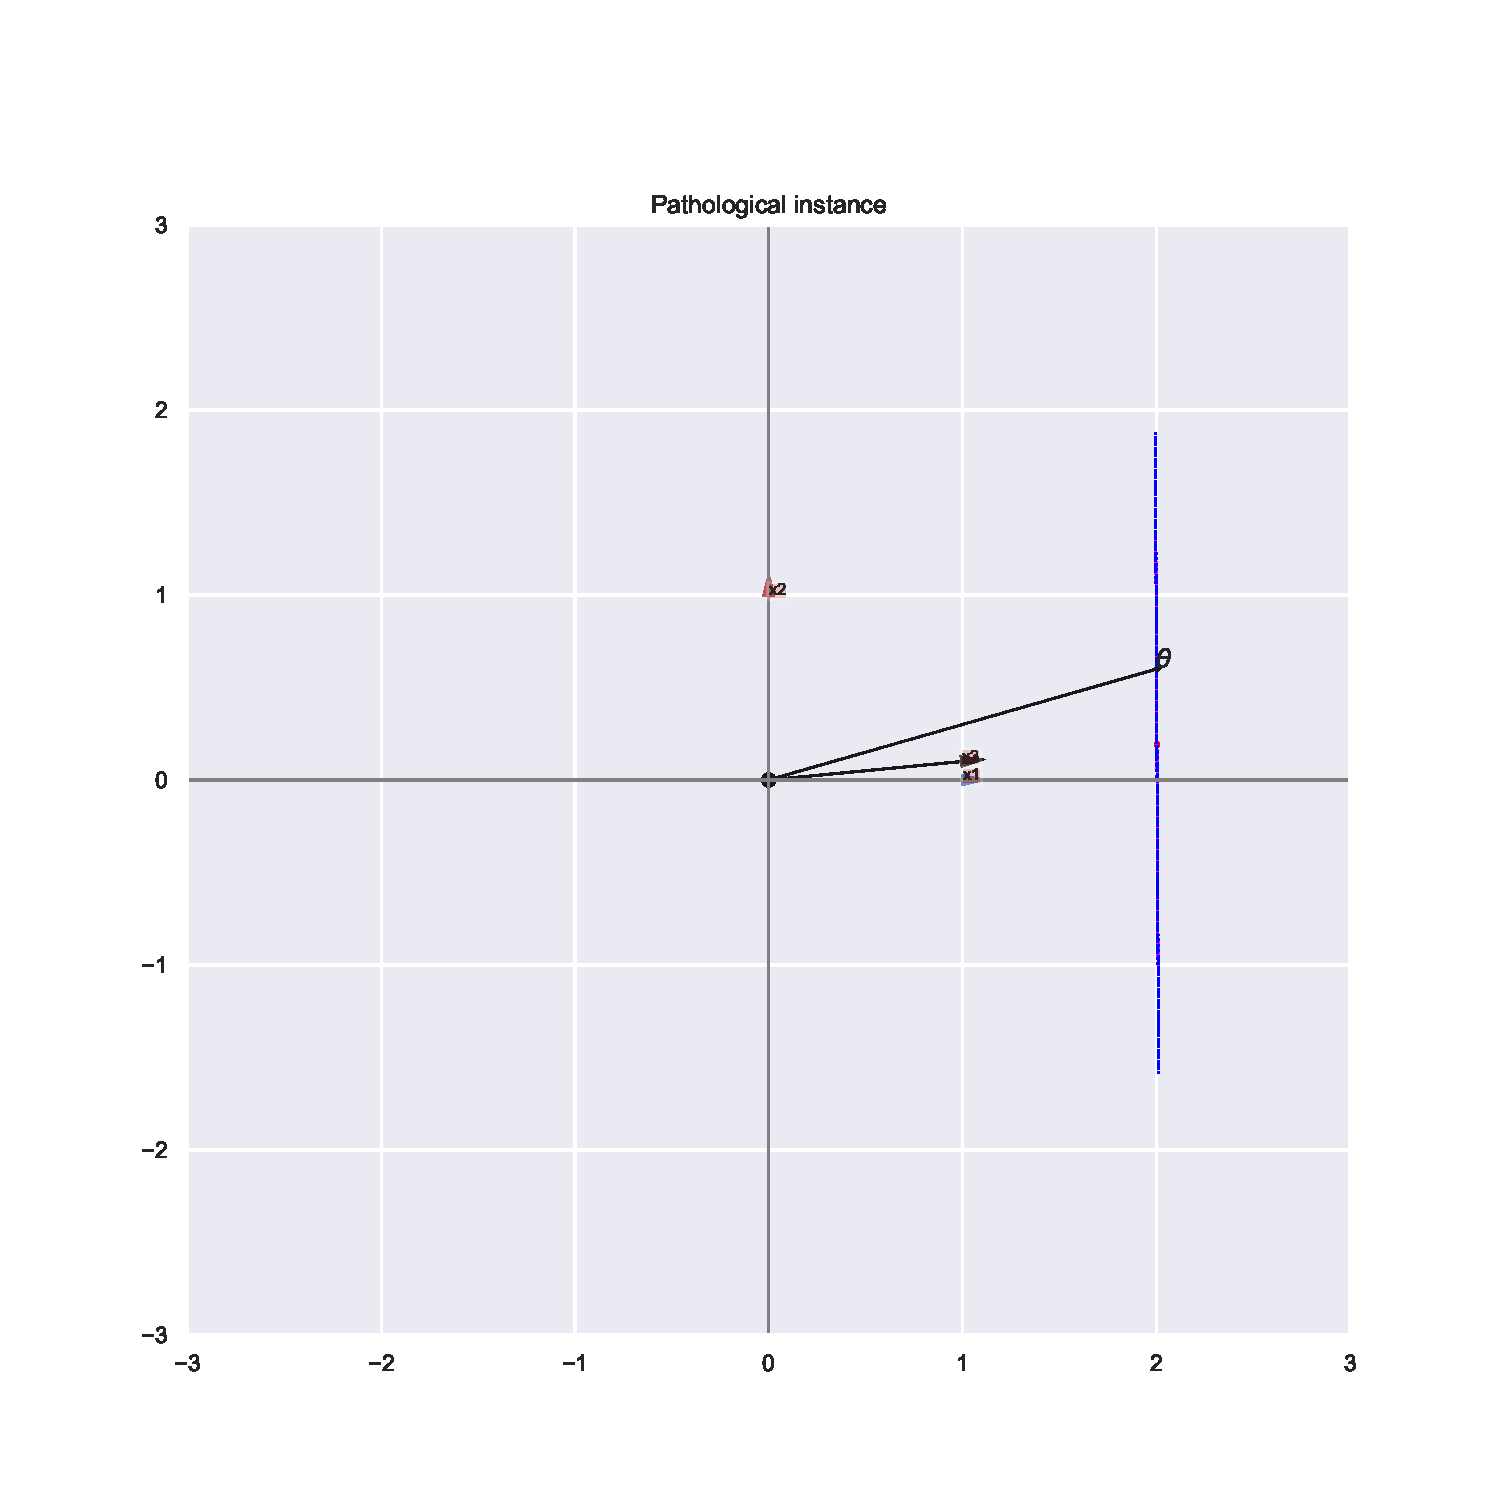
\includegraphics[width=0.55\textwidth]{Chapter4/img/instance.pdf}
    \caption{A pathological problem instance for linear best-arm identification.}
    \label{fig:instance}
\end{figure}

\subsection{A "greedy" fix of \LTCC{}}\label{sec:lgc.bayesian.fix}

In order to overcome the previous issue, one can think of the following greedy version of $\LTCC$. It is inspired by the \emph{greedy} rule already used in (a heuristic version of) \LGapE~\citep{xu2018linear}, and is motivated by the following observation: in order to learn to discriminate between some arm $I^{(1)}$ and a challenger $I^{(2)}$, it may be more informative to select another arm. More specifically, the arm from which a new pull would reduce the most the variance in the estimation of $\bx_{I^{(1)}} - \bx_{I^{(2)}}$. In a standard bandit, this is simply the least pulled arm between $I^{(1)}$ and $I^{(2)}$, but in the linear case it may be another arm! 

\begin{algorithm}[ht]
\centering
\caption{Sampling rule (\LTCCG)}
\label{alg:lt3cg}
%\footnotesize
\begin{algorithmic}[1]
    %(and the $W_n$ function for \textcolor{red}{\TCC})
   %\STATE {\bfseries Initialization:} $\forall \blambda\in\Omega, S_{\blambda}=0, F_{\blambda}=0$
   \For{$n \leftarrow 1,2,\cdots$}
        \State \text{sample} $\btheta_1 \sim \Pi_n$
        \State $\hat{\bx}^{(1)} \leftarrow \argmax_{\bx\in\cX} \bx\transpose\btheta_1$ \text{(indexed by $I^{(1)}$)}
	        \State $I^{(2)} \leftarrow \argmin_{i\neq I^{(1)}}W_n(I^{(1)},i)$ \text{(see \eqref{def:transportation} for the definition)}\Comment{$I^{(2)} \leftarrow \hat{\bx}^{(2)}$}
		    \State \text{evaluate arm} $\hat{\bx} \eqdef \argmin_{\bx\in\cX} \normm{\hat{\bx}^{(1)} - \hat{\bx}^{(2)}}_{(\bA_{\bX_n}+\bx\bx\transpose)^{-1}}$
	    \State \text{update mean and variance according to \eqref{eq:update_mean} and \eqref{eq:update_variance}}
	    \State $n = n+1$
   \EndFor
\end{algorithmic}
\end{algorithm}

\subsection{\texorpdfstring{\LGapE}{} versus \texorpdfstring{\LTCCG}{}: Is one of them optimal?}\label{sec:lgc.bayesian.check}

Upon close examination, \LGapE and \LTCCG are very similar: they both rely on the computation of a leader and a challenger followed by the greedy rule to decide which arm to explore/play, and they actually use the same stopping rule (up to possible tuning of the threshold). The differences are:
\begin{itemize}
    \item how they define the challenger once the leader is chosen;
    \item how they perform exploration: \LGapE{} performs exploration in the choice of the challenger, which depends on some confidence bounds. \LTCCG{} performs exploration in the choice of the leader, which is determined by Thompson sampling.  
\end{itemize}

Table~\ref{tab:comparison} provides a more detailed comparison of the two algorithms for linear bandits. We see in particular that the stopping rule coincide up to the choice $C_n = \sqrt{2\beta(n, \delta)}$.

\begin{table}[ht]
\centering
    %\hspace{-1cm}
    \resizebox{\textwidth}{!}{%
    \begin{tabular}{|c|c|c|}
    \hline 
      &  \LGapE & \LTCCG  \\
      \hline 
      Leader & $I_n^{(1)} = \argmax_{i}\bx_i\transpose\hat{\btheta}_n^{\lambda}$   &   $I_n^{(1)} = \argmax_{i} \bx_i\transpose\tilde{\btheta}_n$ \\
      & with $\hat \btheta_n^{\lambda}$ the least square estimate & with $\tilde{\btheta}_n \sim \mathcal{N}(\hat \btheta_n^\lambda,\hat{\bSigma}_n)$ \\
      \hline
        Challenger & $I_n^{(2)} = \underset{j \neq I_n^{(1)} }{\argmax} \ \left(\bx_j - \bx_{I_n^{(1)}}\right)\transpose \hat{\btheta}_n^\lambda + \normm{\bx_j - \bx_{I_n^{(1)}}}_{\hat{\bSigma}_n} C_n$    &   $I_n^{(2)} = \underset{j \neq I_n^{(1)} }{\argmin} \ddfrac{\left( \left(\bx_j - \bx_{I_n^{(1)}}\right)\transpose \hat\btheta_n^\lambda\right)^2}{2\normm{\bx_j - \bx_{I_n^{(1)}}}_{\hat{\bSigma}_n}^2} \1\left\{\bx_{I_n^{(1)}}\transpose\hat\btheta_n^\lambda \geq \bx_{j}\transpose\hat\btheta_n^\lambda\right\}$ \\
      \hline
          Stopping & $ \left(\bx_{I_n^{(2)}} - \bx_{I_n^{(1)}}\right)\transpose \hat\btheta_n^\lambda + \normm{\bx_{I_n^{(2)}} - \bx_{I_n^{(1)}}}_{\hat\bSigma_n} C_n < 0$    &  $\underset{j \neq J_n^{(1)} }{\min} \ddfrac{\left( \left(\bx_j - \bx_{J_n^{(1)}}\right)\transpose \hat\btheta_n^\lambda\right)^2}{2\normm{\bx_j - \bx_{J_n^{(1)}}}_{\hat{\bSigma}_n}^2} \1\left\{\bx_{J_n^{(1)}}\transpose\hat\btheta_n^\lambda \geq \bx_{j}\transpose\hat\btheta_n^\lambda\right\} > \beta(n,\delta)$ \\
                 & $ \Leftrightarrow \ddfrac{\left(\left(\bx_{I_n^{(1)}} - \bx_{I_n^{(2)}}\right)\transpose \hat\btheta_n^\lambda\right)^2}{2\normm{\bx_{I_n^{(2)}} - \bx_{I_n^{(1)}}}_{\hat\bSigma_n}^2} > C_n^2/2$    &   $\Leftrightarrow J_n^{(1)} = \argmax_{j} \bx_j\transpose\hat{\btheta}_n^\lambda, \ \ddfrac{\left(\left(\bx_{J_n^{(1)}} - \bx_{J_n^{(2)}}\right)\transpose \hat\btheta_n^\lambda\right)^2}{2\normm{\bx_{J_n^{(2)}} - \bx_{J_n^{(1)}}}_{\hat\bSigma_n}^2} > \beta(n,\delta)$ \\
          \hline
    \end{tabular}%
    }
\caption{Comparison between the two algorithms.} \label{tab:comparison}
\end{table}

\paragraph{Experiments for classical bandits.}
\LTCCG can be particularized to the classic BAI setting (that corresponds to choosing the canonical basis as contexts). In that case, the selection rule in Line 6 of Algorithm~\ref{alg:lt3cg} corresponds to choosing the least pulled arm between the two candidates. 

We investigate whether \LTCCG{} could be optimal in the classical bandit setting with some experiments. In particular, we call the derived algorithm \TCCG{}. See Fig.~\ref{fig:convergence} for a comparison against the asymptotically optimal \DT rule and the oracle. It is seemingly that \LTCCG{} is not very promising for being asymptotically optimal.

\begin{figure}[ht]
    \centering
    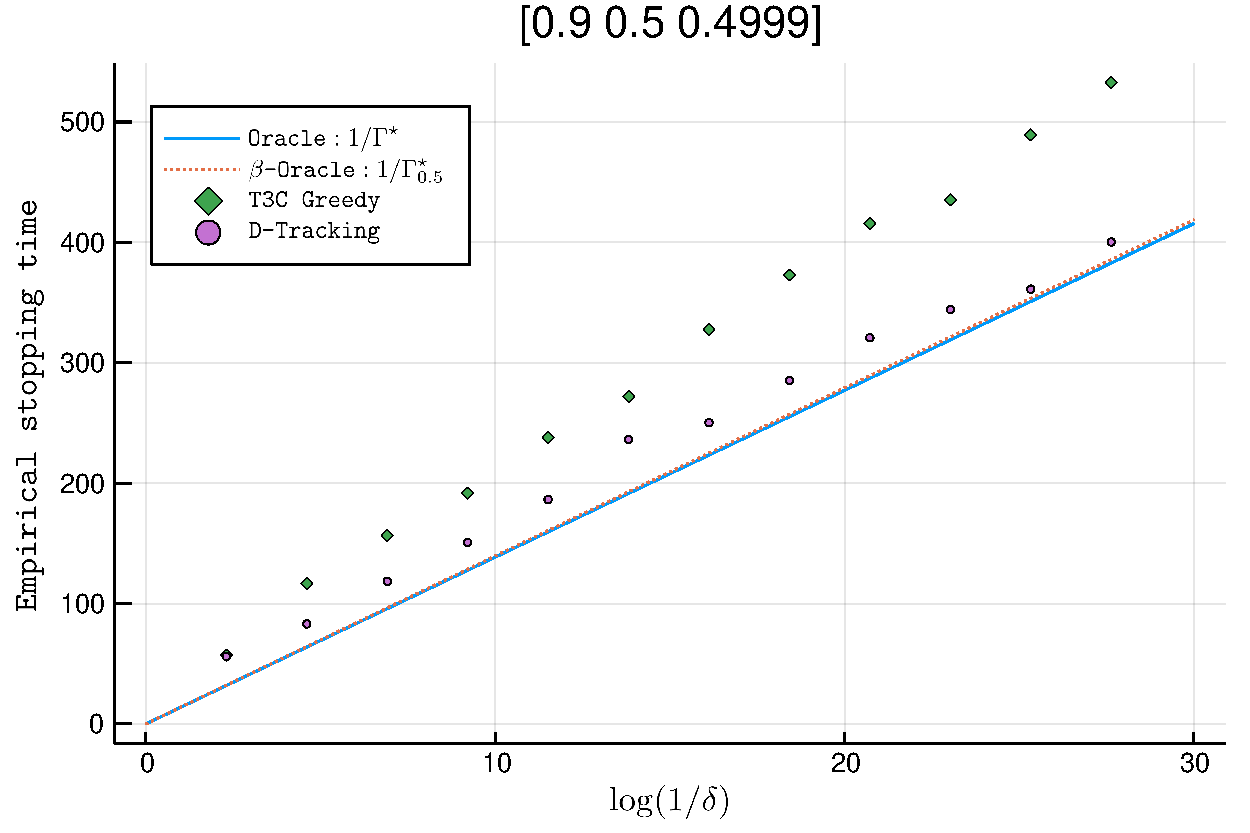
\includegraphics[width=0.33\textwidth]{Chapter4/img/res1.pdf}
    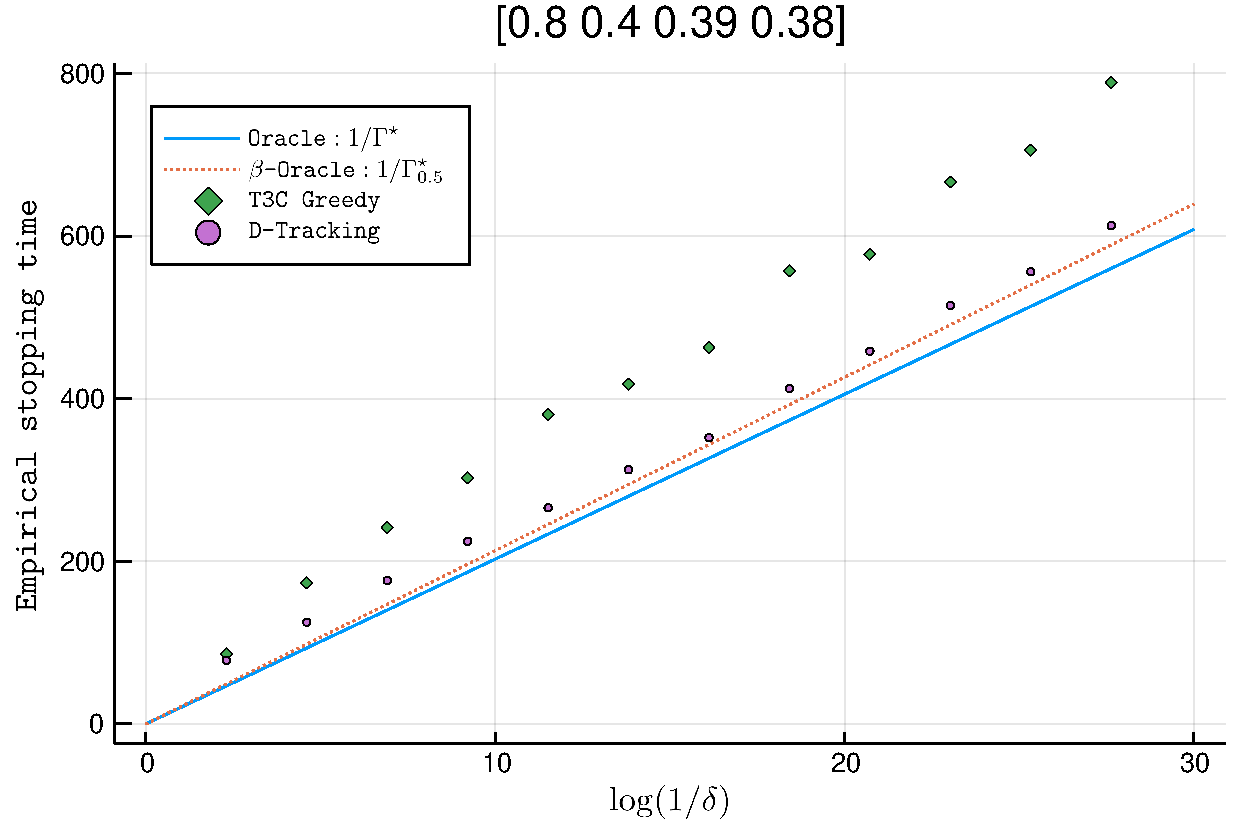
\includegraphics[width=0.33\textwidth]{Chapter4/img/res2.pdf}
    \caption{\TCCG{} versus \Track{} for different value of $\delta$.}
    \label{fig:convergence}
\end{figure}

\subsection{Empirical performance of \LTCCG{}}
\paragraph{Results.}
We compare the performance of \LTCCG{} to \LGapE{} over the aforementioned pathological instance with $d=2$, $c=2$ and two values of $\alpha$. More precisely, we report in Table~\ref{table:pulls1} the total number of pulls and also the number of pulls allocated to each arm for each of the sampling rules. The results confirm our intuition in the previous section. 

\begin{table}[ht]
\centering
\begin{tabular}{|c|c|c|}
 \hline
 & \LTCCG & \LGapE \\
 \hline
 \textbf{$\bx_1=(1,0)\transpose$} & $1783.1$ & $5844.4$ \\
 \hline
 \textbf{$\bx_2=(0,1)\transpose$} & $357009.0$ & $1169260.5$ \\
 \hline
 \textbf{$\bx_3=(\cos(0.01),\sin(0.01)\transpose)$} & $1.0$ & $1.0$ \\
 \hline
 \textbf{Total} & $\textbf{358793.1}$ & $1175105.9$ \\
 \hline
\end{tabular}
\caption{Average number of pulls of each arm ($d=2, \delta=0.1$).}
\label{table:pulls1}
\end{table}

\begin{table}[ht]
\centering
\begin{tabular}{|c|c|c|c|}
 \hline
 & \LTCC ($\beta=1/2$) & \LTCCG & \LGapE \\
 \hline
 \textbf{$\bx_1=(1,0)\transpose$} & $131.3$ & $24.9$ & $26.3$ \\
 \hline
 \textbf{$\bx_2=(0,1)\transpose$} & $3.3$ & $60.8$ & $63.4$ \\
 \hline
 \textbf{$\bx_3=(\cos(\pi/4),\sin(\pi/4)\transpose)$} & $133.4$ & $1.0$ & $1.0$ \\
 \hline
 \textbf{Total} & $268.0$ & $\textbf{86.7}$ & $89.7$ \\
 \hline
\end{tabular}
\caption{Average number of pulls of each arm ($d=2, \delta=0.1$).}
\label{table:pulls2}
\end{table}

We also compare the impact of the dimension $d$ over the performance of our sampling rule and $\LGapE$. We run experiments on the same instance with a value of the angle set to $\alpha=0.1$. This time we let the dimension $d$ varying from 2 to 6. \LTCC{} is always better and the performance gap increases with the dimension. Thus, our algorithm seems to be more robust to the dimension.

\begin{figure}[ht]
    \centering
    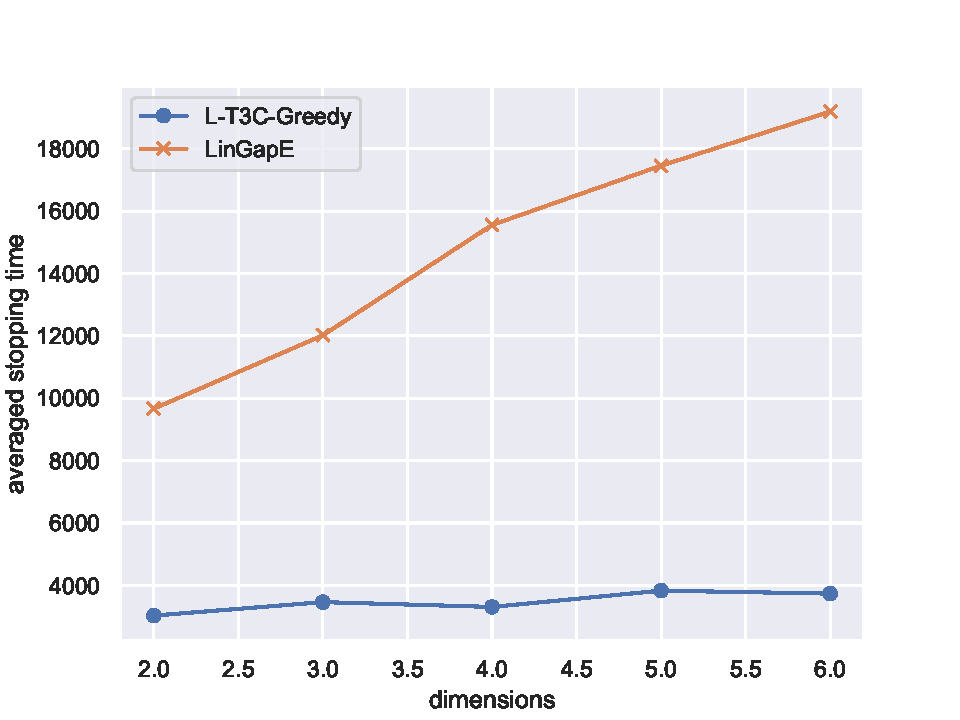
\includegraphics[width=0.5\textwidth]{Chapter4/img/dims.pdf}
    \caption{Comparison of the sample complexity of \LTCCG{} and \LGapE{} on the pathological instance in $\R^d$ for different values of $d$.}
    \label{fig:dims}
\end{figure}

\paragraph{Rank-1 multivariate normal distribution sampling.}
A technical point for the experiments in this section is to sample from a multivariate normal distribution (e.g. for \LTCC{}). We can proceed by the following.

Indeed, a random Gaussian vector 
\[
    \bX = (X_1, X_2, \ldots, X_d)\transpose
\] 
of mean vector $\bar{\bmu}$ and covariance matrix $\bSigma$ can be formally defined as following,
\[
    \bX \sim \cN(\bar{\bmu}, \bSigma) \iff \exists \bar{\bmu}\in\mathbb{R}^d,\bA\in\mathbb{R}^{d\times d'} \ \text{s.t.} \ \bX = \bA \mathbf{Z} + \bar{\bmu},
\]
for $Z_i \sim\ \mathcal{N}(0, 1)$ i.i.d. with $i\in\{1,\ldots,d'\}$, and here $\bSigma = \bA\bA\transpose$.

To draw a sample from a multivariate normal distribution, according to the previous definition, one can first find any real matrix $\bA$ such that $\bA\bA\transpose = \bSigma$. Then draw a vector $\bZ$ whose components independently follow standard normal distribution. Finally $\bX = \bA \mathbf{Z} + \bar{\bmu}$ forms a valid sample. The main issue is thus how to find an appropriate matrix $\bA$.

In this section, we need to sample from $\cN(\hat{\btheta}^\lambda_n,\hat{\bSigma}_n)$, where the covariance matrix $\hat{\bSigma}_n$ is a positive-definite matrix. A usual way is to apply the Cholesky decomposition, which is computationally inefficient if it were to be applied at each time step. Fortunately, we can apply rank-1 Cholesky decomposition in our case.  

%We, however, notice that $\bA = (\hat{\bSigma}_n)^{1/2}=\sigma(\bB^{\lambda}_n)^{-1/2}$ is also a valid candidate, and is thus can be also updated iteratively using a similar formula to the Sherman-Morrison formula.

%More precisely, we have
%\begin{align*}
%    \forall t\geq 0, \quad (\bB^{\lambda}_{t+1})^{-\frac{1}{2}} = (\bB^{\lambda}_t)^{-\frac{1}{2}} - \ddfrac{\left(1-\sqrt{1-\frac{\normm{\hat{\bx}_{t+1}}_{(\bB^{\lambda}_t)^{-1}}^2}{1+\normm{\hat{\bx}_{t+1}}_{(\bB^{\lambda}_t)^{-1}}^2}}\right)}{\normm{\hat{\bx}_{t+1}}_{(\bB^{\lambda}_t)^{-1}}^2} (\bB^{\lambda}_t)^{-\frac{1}{2}}\hat{\bx}_{t+1}\hat{\bx}_{t+1}\transpose(\bB^{\lambda}_t)^{-\frac{1}{2}}.
%\end{align*}

% \subsection{Technical tools}

% \subsection{Tail bounds}
% Following are the classic Gaussian tail bound inequalities written in our linear context (see e.g.~\citealt{qin2017ttei} for detailed proofs).

% \begin{lemma}\label{lemma:tail_upper}
% For any $i,j\in\{1,\ldots,K\}$, if $\bx_i\transpose\hat{\btheta}^\lambda_n<\bx_j\transpose\hat{\btheta}^\lambda_n$,
% \begin{align}
%     \Pi_n\left[\bx_i\transpose\btheta>\bx_j\transpose\btheta\right] &\leq \frac{1}{2} \expp{-\frac{\left(\bx_j\transpose\hat{\btheta}^\lambda_n-\bx_i\transpose\hat{\btheta}^\lambda_n \right)^2}{2\normm{\bx_i-\bx_j}_{\hat{\bSigma}_n}^2}}.
% \end{align}
% \end{lemma}

% \begin{lemma}\label{lemma:tail_lower}
% For any $i,j\in\{1,\ldots,K\}$, if $\bx_i\transpose\hat{\btheta}^\lambda_n<\bx_j\transpose\hat{\btheta}^\lambda_n$,
% \begin{align}
%     \Pi_n\left[\bx_i\transpose\btheta>\bx_j\transpose\btheta\right] &\geq \frac{1}{\sqrt{2\pi}} \expp{-\frac{\left(\bx_j\transpose\hat{\btheta}^\lambda_n-\bx_i\transpose\hat{\btheta}^\lambda_n +\normm{\bx_i-\bx_j}_{\hat{\bSigma}_n}\right)^2}{2\normm{\bx_i-\bx_j}_{\hat{\bSigma}_n}^2}}.
% \end{align}
% \end{lemma}
